\section{Structure of a Remixing System} 
I plan to study the sociotechnical architecture of the Scratch Online Community by examining its following structural attributes (Figure~\ref{fig:structure}):
1) granularity of the remixable components, 
2) modularity of the remixable components, 
3) decomposability of finished projects, 
4) attributability mechanisms and 
5) openness to remix across systems.

In this proposal I briefly define each structural attribute using one or two examples and I explain how I am planning to go about studying it.
I plan to do analyze these structural properties of the system using varied approaches including:
1) case studies that give an rich description of different scenarios that elucidate on the influence of each attribute,
2) analyses the data corpus to understand the frequency of the scenarios and the relationships between the structural attributes,
3) natural design experiments to study the effect of varying some of the structural dimensions.

\begin{figure} 
\centering
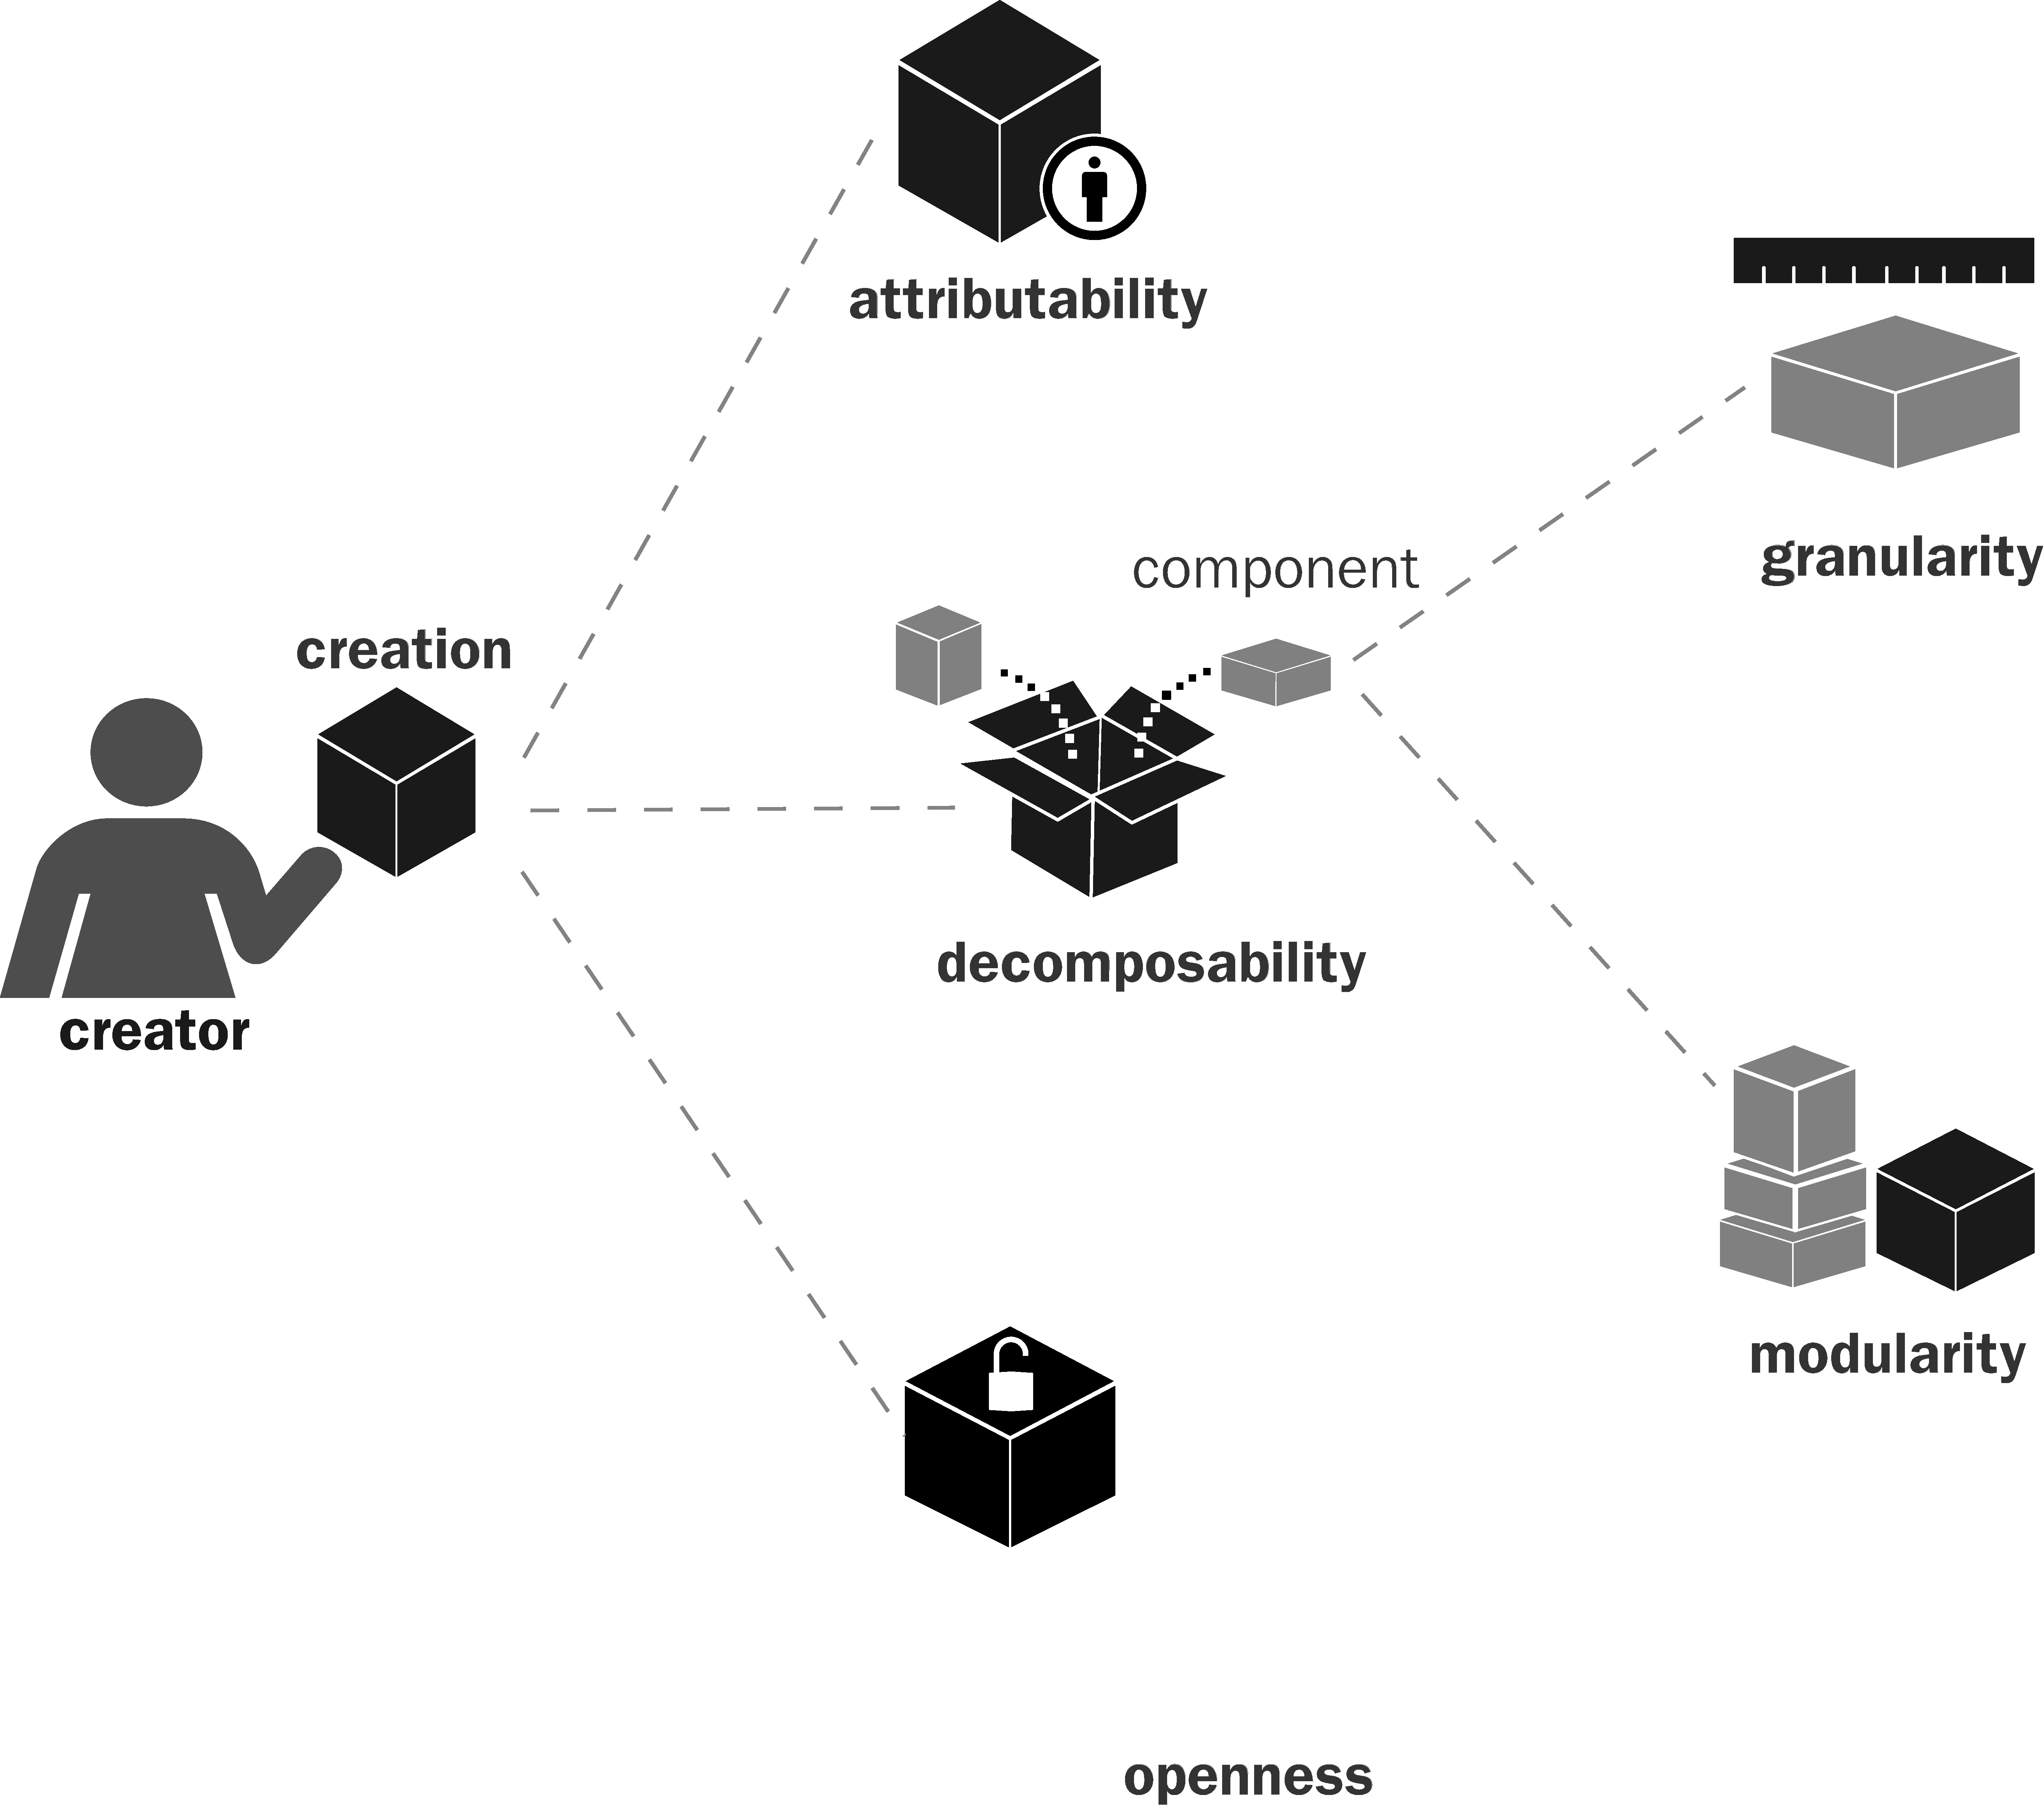
\includegraphics[width=3.25in]{figures/structure.pdf}
\caption{Structural dimensions of a remixing system}
\label{fig:structure}
\end{figure}

\subsection{Granularity}
Granularity is the size of projects' modules \citet{benkler_coases_2002}. 
In Scratch, projects have a couple levels of granularity.
Projects are made up of ``sprites'', for example, characters in a game or a elements in the user interface elements of an interact simulations.
Each sprite can have ``scripts'' or  stacks of programming blocks that control the sprite's behavior such as its position on the screen, its looks, sounds and interaction with other sprites and the user (via mouse, keyboard, or other sensors).
Each sprite also has one or more costumes or images that represent the different visual states of a sprite.
Sprites can also have sounds that are played programmatically, for example, a character in a game could make a sound each time it jumps.

\subsubsection{Proposed work}
The Scratch Online Community, by default it only allows for sharing at the coarsest degree of granularity: only projects can be shared. 
I plan to analyze the implications of this design decision and the ways  people get around the limitations of the architecture.

I have anectdotal evidence that Scratch participants get around the granularity limitations by sharing full projects with the sole intention of sharing a single sprite, script, image or sound.
This need for finer granularity often stems from a desire to engage in sharing practices that the original design did not anticipate. For example, I have documented before the existence of ``coloring contests'' \citep{nickerson_appropriation_2011} where Scratch community remix in order to add color to an image. or as part of group collaboration.
I plan to look these practices in more detail to understand the ways in which a finer granularity mechanisms would help support different types of creative and collaborative learning practices beyond the the existing research that suggests that finer granularity is correlated to the number of people engaged in cooperative activities.

In order to analyze the effect of explicitly supporting finer degree of granularity through a natural experiment, I plan to analyze the adoption ``Scratch Resources'' \footnote{Available at http://resources.scratchr.org}, a website created by members of the Scratch community to support sharing sprites, images and sounds. 
% TODO link to Von Hippel at al on user innovation

Some of my motivating questions are: 
how common is sharing and remixing across the different levels of granularity available (even if not explicitly supported)?
what are the types of participants and motivations for sharing finer grained components?
what role does granularity play in the likelihood of a project being remixed controlling for all other factors?
how do different levels of granularity impact the type and quality of remixes?
how do different levels of granularuty support different levels of familiarity with Scratch, that is, are novices more likely to rely on coarser granularity when engaging in remixing as a scaffolding mechanism?

\subsection{Modularity}
\citet{benkler_coases_2002} defines modularity as the ``property of a project referring to the extent to which it can be broken down into smaller components, or modules, that can be independently and asynchronously produced before they are assembled into a whole.''
For the purpose of this work, I will separate two different aspects of modularity:
1. The ease of \emph{integrating} such components into new creations or remixes.
2. The ease of \emph{decomposing} an existing project into smaller components, typically for the purpose of remixing.
In this section I plan to analyze the term ``modularity'' by focusing on the first aspect.
In the next section, I will focuson the second aspect under the term ``decomposability''.

\subsubsection{Proposed Work}
There are some components or projects that can be more easily integrated into new projects. 
One of the questions I am intersted in exploring is what makes some components more modular than others.

For example, an image generated programmatically might be harder to integrate than one in bitmap format. 
A module that representing a cultural icon, such as Mario\footnote{Mario is a character in a popular video game called Mario Bros. from Nintendo Inc.}, is perhaps easier to integrate into other projects than an image of a less well-known character.
However, there are situation when new subcultural icons emerge within the Scratch community.
For example, a character called Maki-Tak created by a community member from New Zealand started a whole genre of projects, called Takis.
These projects use adaptations of that lizard. 
% Other examples: Mr happy Man
There are also situations where some components are remixed despite their internal complexity which might indicate that these could be built in a way that their internal complexity is hidden and remixing them is easy. 
For example there is a sprite created by an advanced Scratch user that represented a physics simulation of a string. 
This project was later remixed in a project where it represented a necklace.

I plan to operationalize the assessment of modularity by measuring its adoption through number of remixes.
The assumption will be that more modular components are remixed more.
I will examine this in two types of components:  ``samples'' and ``community-generated''.
% Sample components are those that come pre-installed with Scratch. For example, sample images, sounds, sprites and projects in some cases.
% Community-generated are those created by end-users.
For example, ``jetpack girl'' is a sample script consisting of five costumes and  sounds for a flying character that can be controlled with the keyboard.
The code of the sprite comes with an invitation to remix: ``Import me into your own project'' and an explanation on how to use it ``arrow keys make me fly''.
These sample components are not only sprites, there are also hundreds of images and sounds that come with Scratch such as photos of people, animals, things, etc.
In addition to these sample components, there are thousands of components created by community members that are remixed and that can be found in places like Scratch Resources and Scratch projects that explicitly state that they include sprites, images and sounds for others to reuse.

The type of questions I will try to answer are then are:
1. What technical or cultural attributes are linked with component modularity? 
2. Are more modular components used more often by newcomers and do they provide scaffolding in their learning of Scratch programming?
3. Are community-generated components more often created by advanced users?

\subsection{Decomposability}
Building on the concept of modularity examined before, in this section I will examine decomposability as the ease of decomposing a compiled project.
Decomposability is the ease of breaking something apart for the purpose of remixing it.
Therefore decomposability depends on the internal complexity of a project, which in itself is dependent on the expertise of the person attempting to decompose the project.
For example, one can argue that images in Flickr.com are harder to decompose than those in OpenClipart.org, which provides the source vectors, or Aviary.com which provides the bitmap images that were used to create an image.
The same happens with software applications that provide the source code in contrast with thost that only provide the final compiled executable.
But even if the source is provided, there are some cases where projects are ``impenetrable'' due to their complexity or a missmatch between the expertise of the person trying to decompose a project and the complexity of the project. 
For example, for a novice programmer having access to the source code of the Linux kernel might not allow for easy decomposability.

In Scratch, all the sources of a project are provided so the decomposablity of a project depends, among other things, more on how interconnected its different components are. 
For example, sometimes sprites ``broadcast'' messages back and forth making their decomposablity much harder than those that are self-contained.
Also, some creators add instructions to their projects explaining how they can be broken apart, while others obfuscate their code to prevent remixing.

\subsubsection{Proposed Work}
I will first do a manual analysis of a sample projects to observe patterns of decomposability. 
Using the findings of this analysis I will come up with mechanisms to automate the evaluation of decomposability. 
For example, it is possible that a decomposability metric could depend on the use of particular blocks (the ``broadcast'' block could reduce its ranking, while comments in the code would increase it), explicit obfuscation or matching between the average expertise level of community members and the expertise required to understand a project.

I will also look at remixes to analyze how different they are from their original project. 
The assumption would be that ``impenetrable'' projects would be correlated with no remixing or to superficial remixes, such as slights changes in the images,
while highly decomposable projects are associated with significant differences betweent the remix and the original.

I will also analyze in detail the practices of code obfuscation and the strategies people use to discourage decomposability of their projects.

\subsection{Attributability}
% Experiments with automatic vs credit. Responses. Results. Previous work. Future work:
% Not always desired attribution.
% - Notes 
% - Creator endorsed attribution.

\subsection{Openness}
% Across systems. Ethos explained. Creative commons version for kids. DeviatnArt conflicts
% 

